\chapter{Estructura del sistema de distribución de carga}
\label{cap:estructuraSistema}
\section{Componentes del sistema}
	Los componentes que se establecen en el sistema de distribución de carga son cuatro: monitor de carga, analizador de carga, predictor de carga y administrador de réplicas, que se pueden apreciar en la Figura \ref{fig:componentesSistemas}. 

\begin{figure}[hb!]
  \centering
    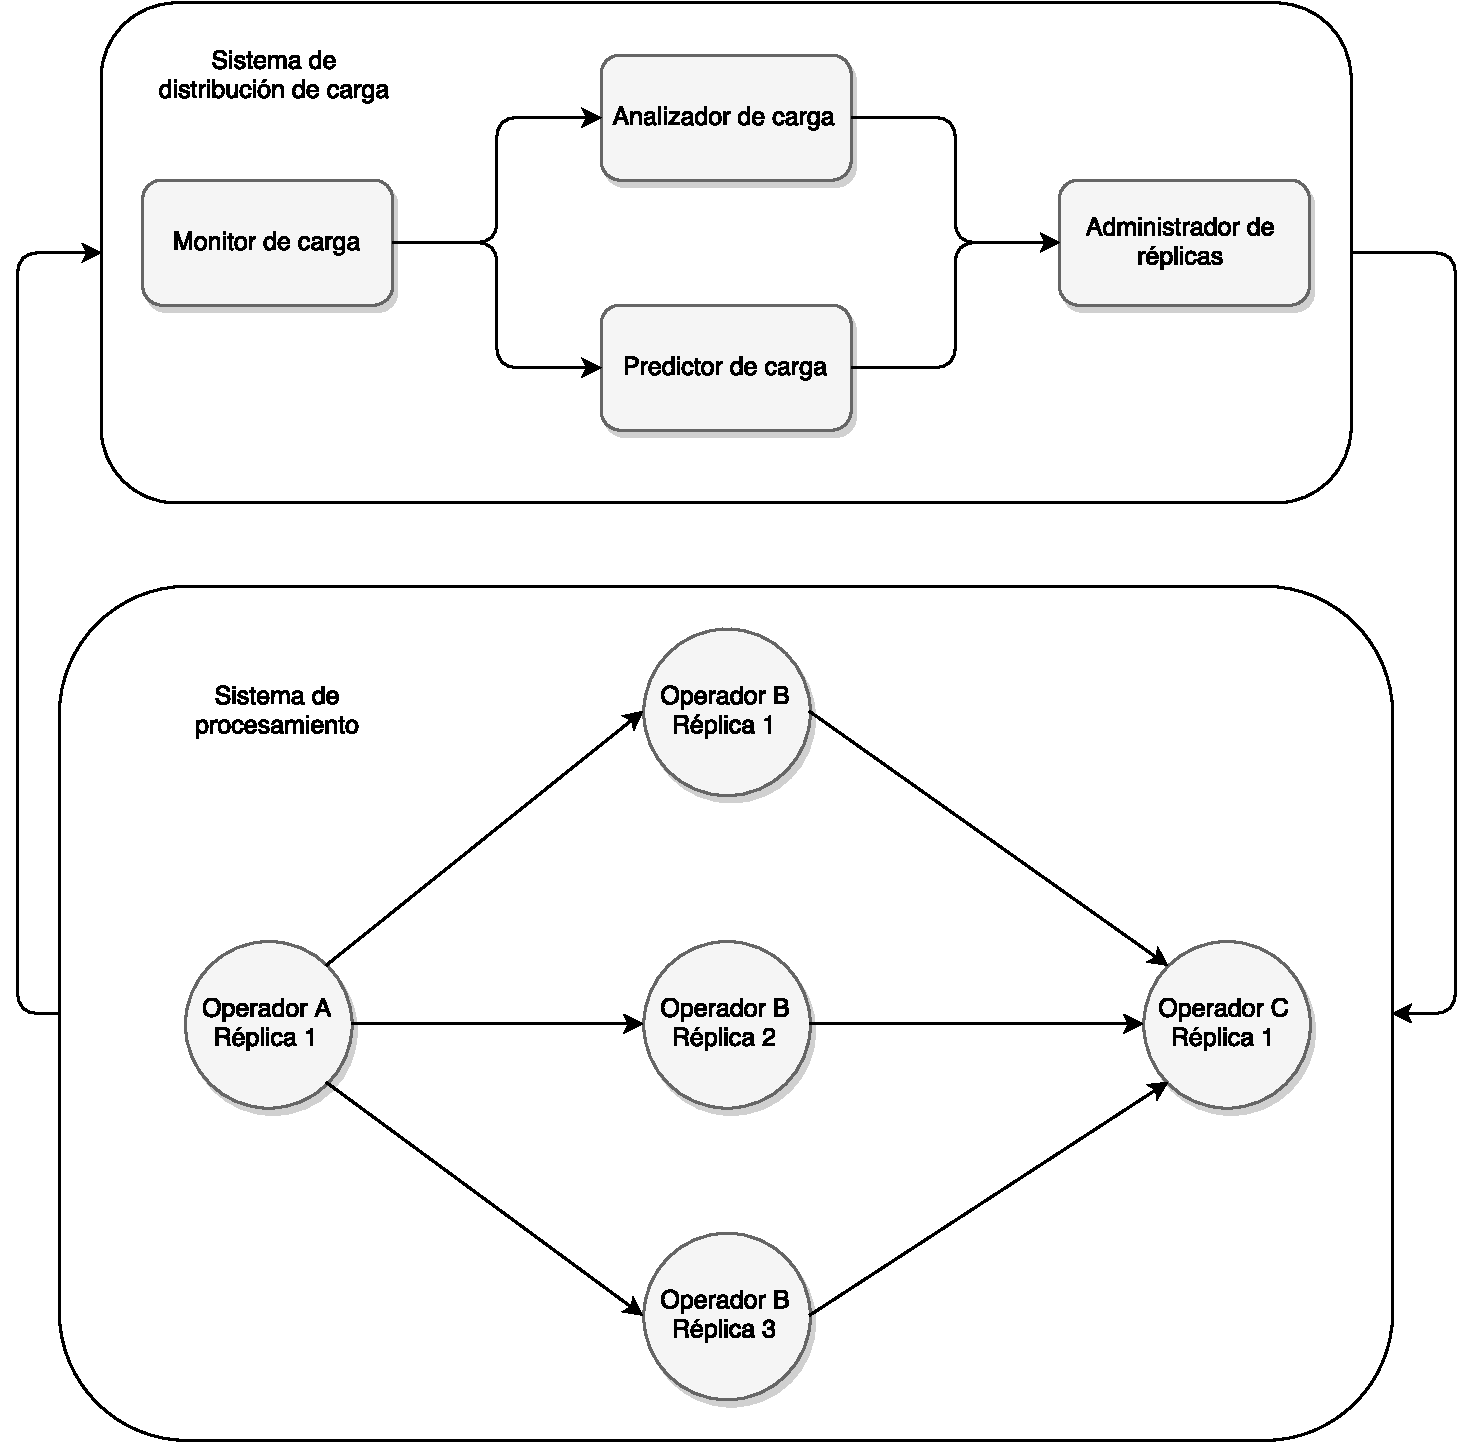
\includegraphics[scale=0.5]{images/Diagrama.pdf}
  \caption{Estructura del sistema de distribución de carga}
  \label{fig:componentesSistemas}
\end{figure}

\subsection{Inicialización del sistema}
	Antes de procesar el flujo de los distintos operadores, es necesario registrar la topología del sistema, por lo tanto cada uno de los operadores son identificados en el monitor de carga, como también la direccionamiento entre los distintos operadores.
	
	%Esto fue implementando dado 

\subsection{Monitor de carga}
	Este componente está a cargo de recopilar las estadísticas de cada uno de los operadores, como la tasa de llegada, de procesamiento y eventos procesados. Para guardar las estadísticas, se utilizó un arreglo de un objeto, cuyo objeto está especificado en la Tabla \ref{tab:statusPE}.
	
\begin{table}[!ht]
\centering
\begin{tabular}{|c|c|c|}
	\hline
	Tipo & Atributo & Definición \\\hline 
	long & recibeEvent & Cantidad de eventos recibidos por el operador \\
	long & sendEvent & Cantidad de eventos enviados por el operador \\
	double & sendEventUnit & Blablabla \\
	double & sendEventPeriod & Blablabla \\
	double & processEvent & Blablabla \\
	long & queueEvent & Blablabla \\
	Queue(Double) & history & Blablabla \\
	Class & pe & Blablabla \\
	int & replication & Blablabla \\
	Queue(Integer) & markMap & Blablabla \\
	long & eventCount & Blablabla \\
	\hline
\end{tabular}
\caption{Estructura del objeto que guarda el estado de un operador.}
\label{tab:statusPE}
\end{table}

Por lo tanto, 